\title{9. Komplexní čísla}
\author{Michaela Dudašková (Jakub Sláma)}
\date{1.5.2025}

\maketitle

\section{Komplexní čísla}

\subsection{Základní definice}
    \begin{itemize}
        \item uspořádané dvojice reálných čísel, značí se $z;z=[a;b]$
        \item skládají se z reálné části $a$ a imaginární části $b$
        \item $\mathbb{C} ....$ množina všech komplexních čísel
    \end{itemize}
    
\subsection{Znázornění komplexních čísel}
    \begin{itemize}
        \item komplexní čísla znázorňujeme v Gaussově rovině
        \item místo osy $x$ a $y$ máme reálnou osu $Re$ a imaginární osu $Im$
    \end{itemize}
    
    \begin{figure}[H]
        \centering
        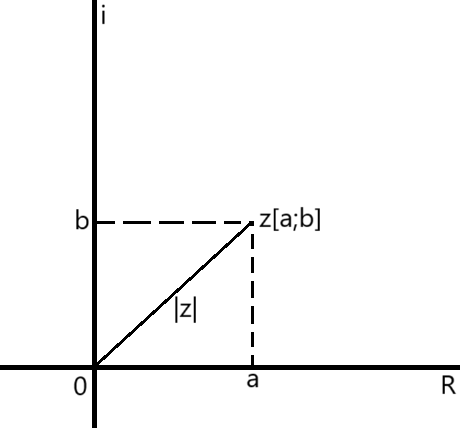
\includegraphics[width=0.2\linewidth]{img/9_graf_komlexniho_cisla.png}
        \caption{Komplexní číslo na grafu s reálnou a imaginární osou}
        \label{fig:enter-label}
    \end{figure}
    
\subsubsection{Typy (podmnožiny) komplexních čísel}
    \begin{itemize}
        \item pokud komplexní číslo $z$ nemá imaginární část ($b=0$), je to \textbf{reálné číslo}
        \item $a=0$ a $b=0$, je to \textbf{nulové číslo}
        \item pokud $a \neq 0$ a $b \neq 0$, je to \textbf{komplexní číslo}
        \item pokud nemá reálnou část ($a=0$), je to \textbf{ryze imaginární číslo}
    \end{itemize}
    
\subsection{Rovnost komplexních čísel}
    $$
        z_1=z_2, a_1=a_2  \wedge b_1=b_2
    $$
    
\subsection{Algebraický tvar komplexního čísla}
    $$
        z=a+bi
    $$
    
\subsection{Imaginární jednotka}
    \begin{itemize}
        \item je to číslo $[0,1]$ a značí se $i$
        \item platí: $i^2 = -1;i^3=-i; i^4=1$
    \end{itemize}
    
\subsection{Součet komplexních čísel}
    $$
        z_1+z_2 = [a_1+a_2;b_1+b_2]
    $$
    $$
        (a+bi)+(c+di) = (a+c) + (b+d)i
    $$
    
\subsection{Součin komplexních čísel}
    $$ 
        z_1 \cdot z_2 = [a_1 a_2 - b_1 b_2,a_1 b_2 + b_1 a_2]
    $$
    $$
        (a + bi)(c + di) = (ac - bd) + (ad + bc)i
    $$
    
\subsubsection{Příklad}
    a)$i^{13}=i^{4 \cdot 3+1}=i$ b)$i^{96}=i^{4 \cdot 24}=1$
    \begin{itemize}
        \item mocninu vydělím 4 a podle zbytku určím výsledek
    \end{itemize}
    
\subsection{Číslo komplexně sdružené a číslo opačné}
    \begin{itemize}
        \item komplexně sdružené číslo se značí $\overline{z}$
    $$
        \textit{číslo } z = [a,b] = a + bi \textit{ a číslo } \overline{z} = [a,-b] = a - bi \textit{ jsou komplexně sdružená}
    $$
        \item součet i součin komplexně sdružených čísel jsou čísla reálná
        \item číslo $-z = -a - bi$ je číslo opačné k číslu $z = a + bi$
    \end{itemize}
    
    
\subsection{Rozdíl komplexních čísel}
    $$
        z_1-z_2=z_1+(-z_2)=(a_1+b_1i)+(-a_2-b_2i)
    $$
    
\subsection{Podíl komplexních čísel}
    $$
        \frac{z_1}{z_2}=\frac{z_1 \cdot \overline{z_2}}{z_2 \cdot \overline{z_2}}=\frac{(a_1+b_1i)(a_2-b_2i)}{(a_2+b_2i)(a_2-b_2i)}=\frac{(a_1a_2-b_1b_2)+(a_2b_1-a_1b_2)i}{a_2^2+b_2^2}
    $$
    
\subsection{Umocňování komplexních čísel}
    \begin{itemize}
        \item druhá a třetí mocnina pomocí vzorečků
    \end{itemize}
    $$
        (a + bi)^2 = (a^2 - b^2) + 2abi
    $$
    $$
        (a + bi)^3 = (a^3 - 3ab^2) + (3a^2b - b^3)i
    $$
\subsection{Absolutní hodnota komplexního čísla}
    \begin{itemize}
        \item vzdálenost komplexního čísla od počátku (bodu $[0,0]$) v Gaussově rovině
    \end{itemize}
    $$
        |z|=\sqrt{a^2+b^2}
    $$
\subsection{Argument (amplituda) komplexního čísla}
    \begin{itemize}
        \item úhel $\varphi$, který svírá kladná poloosa $x$ a absolutní hodnota $z$
    \end{itemize}
    \subsubsection{Určení argumentu přes sinus a kosinus}
        $$
            \cos{\varphi} = \frac{a}{|z|}
        $$
        $$
            \sin{\varphi} = \frac{b}{|z|}
        $$
        \begin{itemize}
            \item rovnice se budou shodovat pro jeden úhel $\varphi$
            \item kvadrant úhlu $\varphi$ odpovídá kvadrantu komplexního čísla v Gaussově rovině
        \end{itemize}
    \subsubsection{Určení argumentu přes tangens}
        $$
            \varphi = \left\{\begin{array}{rcl}
                \arctan{\frac{b}{a}}        & \mbox{pro} & b \geq 0\\
                \arctan{\frac{b}{a}}+\pi    & \mbox{pro} & b < 0
            \end{array}\right.
        $$
\subsection{Goniometrický tvar komplexního čísla}
    \begin{itemize}
        \item komplexní číslo vyjádřeno pomocí argumentu a absolutní hodnoty
    \end{itemize}
    $$
        z=|z|(\cos{\varphi}+i\cdot \sin{\varphi})
    $$
    \subsubsection{Převod z goniometrického tvaru na algebraický tvar}
    \begin{itemize}
        \item vypočítáme funkční hodnoty sinu a kosinu a roznásobíme s absolutní hodnotou:
    \end{itemize}
    
    $$
        \mbox{např.:}\;\; 2(\cos({\tfrac{2}{3}\pi})+i\cdot \sin({\tfrac{2}{3}\pi})) = 2(-\tfrac{1}{2}+\tfrac{\sqrt{3}}{2}i) = -1 + i\sqrt{3}
    $$
\subsection{Moivreova věta}
    \begin{itemize}
        \item pro umocňování - má jeden výsledek
    $$
        z^n=|z|^n(cos(n \cdot \varphi)+i\cdot sin (n \cdot \varphi))
    $$
        \item pro odmocňování - má tolik výsledků, kolikátá je odmocnina ($n$)
    $$
        \sqrt[n]{z}=z_k = \sqrt[n]{|z|} \left( \cos\left( \frac{\varphi + 2k\pi}{n} \right) + i \sin\left( \frac{\varphi + 2k\pi}{n} \right) \right), \quad k = 0, 1, \dots, n-1
    $$
        \item za $k$ dosazujeme čísla $0, 1, 2, \dots, n-1$
        \item získáme výsledky $z_0, z_1, z_2, \dots, z_{n-1}$
    \end{itemize}
    
\subsection{Řešení binomických rovnic}
    \begin{itemize}
        \item pomocí goniometrického tvaru komplexních čísel můžeme řešit i binomické rovnice (rovnice vyšších řádů)(tvar $ax^n+b=0$)
    \end{itemize}
    \subsubsection{Řešení rovnice $x^4 + 16 = 0$}
        
        Rovnici
        $$
        x^4 + 16 = 0
        $$
        převedeme na tvar
        $$
        x^4 = -16.
        $$
        
        Zápis pravé strany v goniometrickém tvaru:
        $$
        -16 = 16 \left( \cos\pi + i\sin\pi \right).
        $$
        
        Použijeme vzorec pro $n$-té odmocniny komplexního čísla:
        $$
        x_k = \sqrt[4]{16} \left( \cos\left( \frac{\pi + 2k\pi}{4} \right) + i \sin\left( \frac{\pi + 2k\pi}{4} \right) \right), \quad k = 0,1,2,3.
        $$
        
        Vypočteme:
        $$
        \sqrt[4]{16} = 2.
        $$
        
        Jednotlivá řešení:
        
        \begin{align*}
        x_0 &= 2 \left( \cos\left( \frac{\pi}{4} \right) + i \sin\left( \frac{\pi}{4} \right) \right) = \sqrt{2} + i\sqrt{2}, \\
        x_1 &= 2 \left( \cos\left( \frac{3\pi}{4} \right) + i \sin\left( \frac{3\pi}{4} \right) \right) = -\sqrt{2} + i\sqrt{2}, \\
        x_2 &= 2 \left( \cos\left( \frac{5\pi}{4} \right) + i \sin\left( \frac{5\pi}{4} \right) \right) = -\sqrt{2} - i\sqrt{2}, \\
        x_3 &= 2 \left( \cos\left( \frac{7\pi}{4} \right) + i \sin\left( \frac{7\pi}{4} \right) \right) = \sqrt{2} - i\sqrt{2}.
        \end{align*}
        
        \textbf{Řešení:}
        $$
        \boxed{
        x = \pm \sqrt{2} \pm i\sqrt{2}
        }
        $$